In the last chapter, we detailed all the methodology steps behind the experimentation. In this one, we will show the proper results obtained by the topic modeling and classification steps.

\section{Topic Modeling}

In this first section, the results are related to the topic modeling step, divided into four stages: the vocabulary selection; the topic coherence optimization; applying LDA in past and present set; and the combination of topics from the past and future.

\subsection{Vocabulary Selection}

After the normalization, we had performed the Luhn's cut in order to remove words with document frequency higher than 60\% and words that appear in less than 5 documents. The cut was performed in both \textit{Past} and \textit{Present} sets, the Table \ref{tab:vocabulary} shows a brief description for the vocabularies dimension before and after the selection, and for their intersection.

\begin{table}[h!]
	\centering
	\caption{Vocabulary description.}
	\label{tab:vocabulary}
	\begin{tabular}{l|cccc}
		\toprule
		          &  \textbf{Raw}  & \textbf{High DF} & \textbf{Low DF} & \textbf{Filtered} \\ \midrule
		Past      & 77512 &   104   & 65480  &  11928   \\
		Present   & 90122 &   183   & 70356  &  19583   \\
		Intersect &   -   &    -    &   -    &   9745   \\ \bottomrule
	\end{tabular}
\end{table}

With this cut, words like ``abstract'', ``show'' and ``reference'' were removed from the vocabulary. They are quite common in this type of scientific publication and are not relevant for analysis. The low frequency includes very specific words and mostly misspellings.

\subsection{Topic Coherence Optimization}

To find the best topic model for our data, an hyperparameter optimization has been performed over the three LDA parameters: $\alpha \in \left\{0.1, 0.5, 1\right\}$, $\beta \in \left\{0.05, 0.1, 0.5, 1\right\}$ and $K \in \left\{10, 15, 20, 25, 30, 35, 40\right\}$. The dataset used was the \textit{Past} set with its vocabulary as described in the previous section. Figure \ref{fig:coherence-optimization} shows the coherence score $C_{\text{V}}$ by the number of topics for the main $\alpha$ and $\beta$ combinations.

\begin{figure}[h!]
	\begin{subfigure}{0.49\textwidth}
		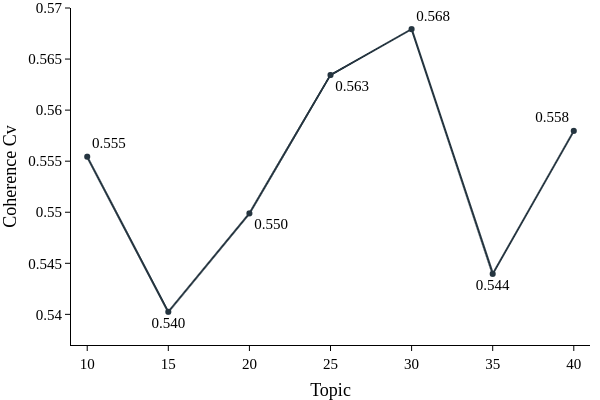
\includegraphics[width=\linewidth]{01.Chapters/05.Results/01_Topic_Cv_A:0.5| B:1.00}
		\caption{$\alpha = 0.5$ and $\beta = 1.0$.}
	\end{subfigure}%
	\hfill
	\begin{subfigure}{0.49\textwidth}
		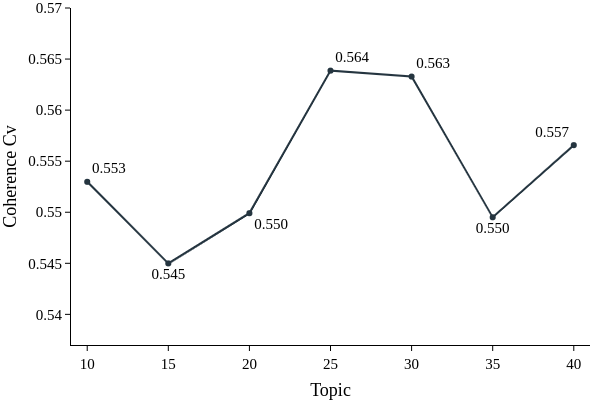
\includegraphics[width=\linewidth]{01.Chapters/05.Results/02_Topic_Cv_A:0.1| B:1.00}
		\caption{$\alpha = 0.1$ and $\beta = 1.0$.}
	\end{subfigure}%
	\vfill
	\begin{subfigure}{0.49\textwidth}
		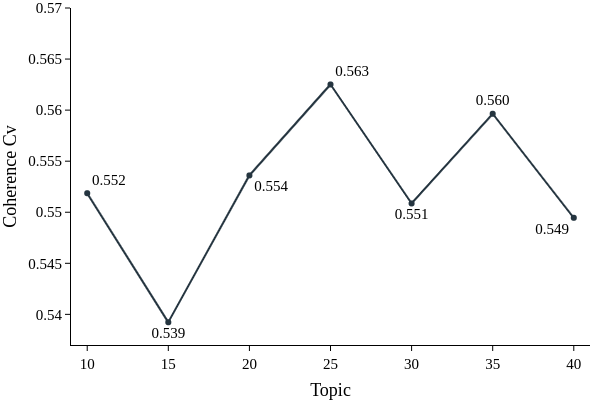
\includegraphics[width=\linewidth]{01.Chapters/05.Results/03_Topic_Cv_A:1.0| B:1.00}
		\caption{$\alpha = 1.0$ and $\beta = 1.0$.}
	\end{subfigure}%
	\hfill
	\begin{subfigure}{0.49\textwidth}
		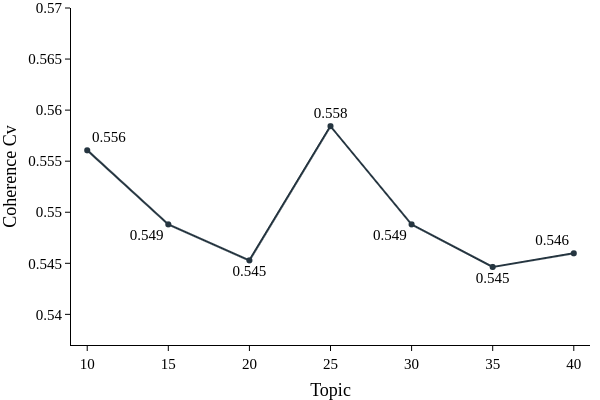
\includegraphics[width=\linewidth]{01.Chapters/05.Results/04_Topic_Cv_A:1.0| B:0.10}
		\caption{$\alpha = 1.0$ and $\beta = 0.1$.}
	\end{subfigure}%
	\caption{Topic Coherence Optimization.}
	\label{fig:coherence-optimization}
\end{figure}

Although the combination for $\alpha = 0.5$ and $\beta = 1.0$ has it maximum for $30$ topics, we can clearly detect a maximum trend for $25$ topics. From the application point of view, the smaller the number of topics the better for a human to follow their evolution. In this manner, we decided on $25$ topics to proceed with the experiment, with this value for $K$, the $\alpha$ and $\beta$ parameters with the best coherence score are $0.1$ and $1.0$, respectively.

\subsection{Finding Topics}

At this stage we had performed the LDA algorithm over the \textit{Past} and \textit{Present} sets, with the parameters established in the previous stage and their respective vocabularies, to find their topics. After the modeling the \textit{Present} model has presented a coherence of $0.614$, this indicates that the \textit{Present} model is slightly better than the \textit{Past} one.

\subsubsection{Past}

Figure \ref{fig:past-wordcloud} shows some word clouds for \textit{Past} topics that are easier to identify what they talk about. For example, topic 0 talks about image recognition, topic 10 clearly is about reinforcement learning, topic 16 can be about supervised learning, and topic 19 about facial recognition. To assess all the topics in more detail check Appendix \ref{apdx:past}.

\begin{figure}[h!]
	\begin{subfigure}{0.49\textwidth}
		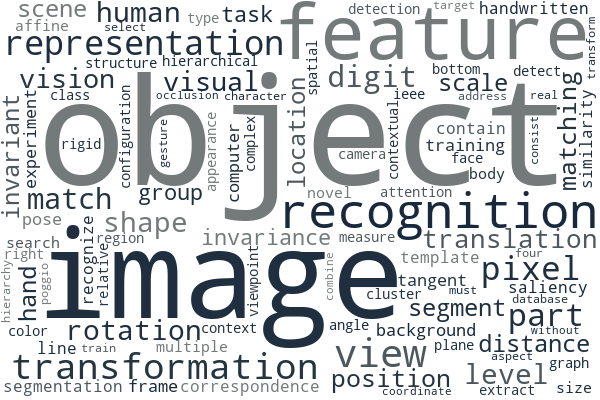
\includegraphics[width=\linewidth]{01.Chapters/05.Results/past_00}
		\caption{Past topic number 0.}
	\end{subfigure}%
	\hfill
	\begin{subfigure}{0.49\textwidth}
		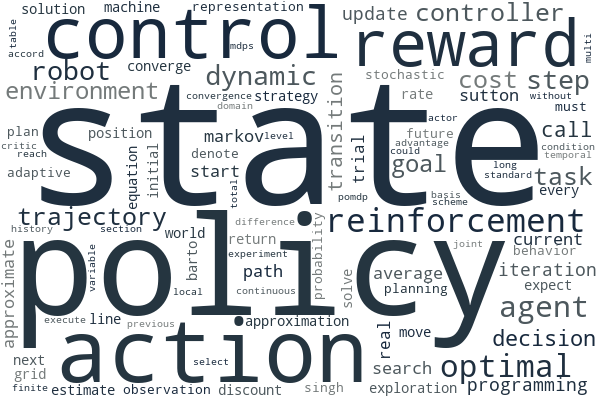
\includegraphics[width=\linewidth]{01.Chapters/05.Results/past_10}
		\caption{Past topic number 10.}
	\end{subfigure}%
	\vfill
	\begin{subfigure}{0.49\textwidth}
		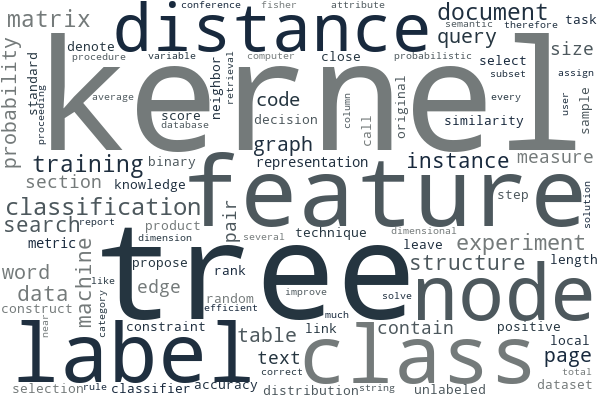
\includegraphics[width=\linewidth]{01.Chapters/05.Results/past_16}
		\caption{Past topic number 16.}
	\end{subfigure}%
	\hfill
	\begin{subfigure}{0.49\textwidth}
		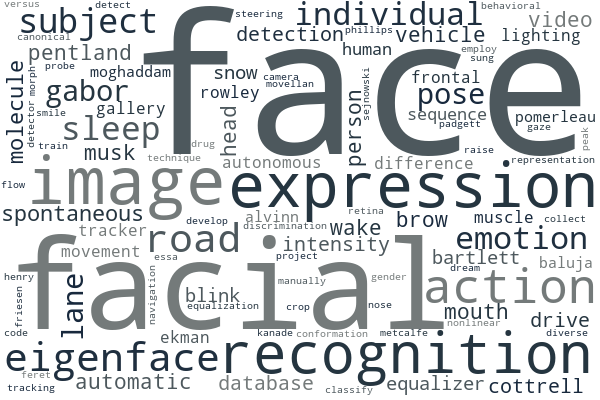
\includegraphics[width=\linewidth]{01.Chapters/05.Results/past_19}
		\caption{Past topic number 19.}
	\end{subfigure}%
	\caption{\textit{Past} topics wordclouds.}
	\label{fig:past-wordcloud}
\end{figure}

Besides getting the topics we also have the distribution of the documents of topics. Using these distributions we had labeled the documents as positive or negative for the topics with a threshold of $1 / K$, i.e., for a document covers a given topic his probability has to be at least $0.08$. This probability guarantees, by the pigeonhole principle, that the documents have at least one topic.

Figure \ref{fig:past-topic-dist} shows the distribution of topics over the documents. In Figure \ref{fig:past-percentage-bar} we have the percentage of documents that is about the 25 past topics, Figure \ref{fig:past-percentage-hist} shows the histogram for these percentages, each bin with $2.5\%$. According to the figures, none of the topics are in more than $50\%$ of the documents, some of them are present in less than $2.5\%$, but mostly they are distributed between $10\%$ and $35\%$.

\begin{figure}[h!]
	\begin{subfigure}{0.49\textwidth}
		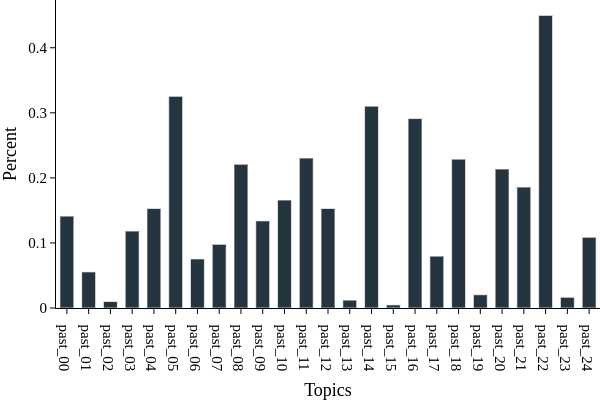
\includegraphics[width=\linewidth]{01.Chapters/05.Results/past-percentage-bar}
		\caption{Percentage of documents with topics.}
		\label{fig:past-percentage-bar}
	\end{subfigure}%
	\hfill
	\begin{subfigure}{0.49\textwidth}
		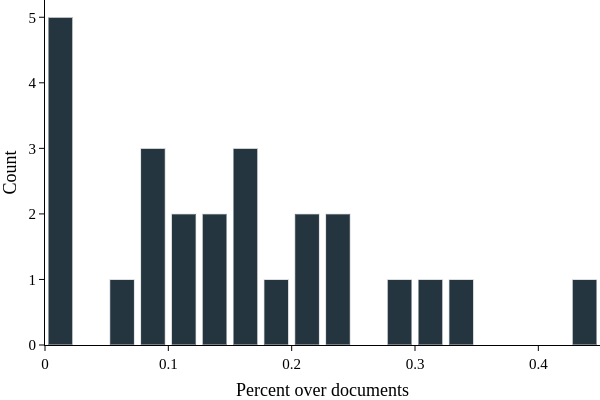
\includegraphics[width=\linewidth]{01.Chapters/05.Results/past-percentage-hist}
		\caption{Histogram for the topic percentages.}
		\label{fig:past-percentage-hist}
	\end{subfigure}%
	\caption{Distribution of topics over the documents.}
	\label{fig:past-topic-dist}
\end{figure}

Figure \ref{fig:past-topic-per-doc} shows the distribution of topics in each document. This histogram shows that most documents have more than one topic, a few have only one topic, even fewer have more than 7, and none document has more than 10 topics.

\begin{figure}[h!]
	\centering
	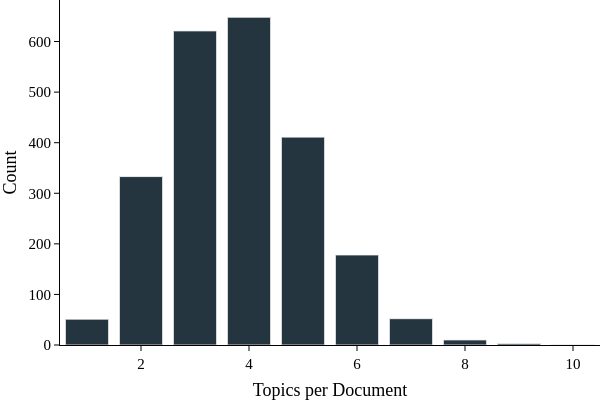
\includegraphics[width=0.6\linewidth]{01.Chapters/05.Results/past-topic-per-doc}
	\caption{Histogram for the number of topics per document.}
	\label{fig:past-topic-per-doc}
\end{figure}


\subsubsection{Present}

Figure \ref{fig:pres-wordcloud} shows some word clouds for \textit{Present} topics that are easier to identify what they talk. For example, topic 0 clearly is about NLP and topic modeling, topic 13 is about clustering, topic 16 can be about statistical inference, and topic 24 about classification. To access all the topics in more detail check Appendix \ref{apdx:present}.

\clearpage
\begin{figure}[h!]
	\begin{subfigure}{0.49\textwidth}
		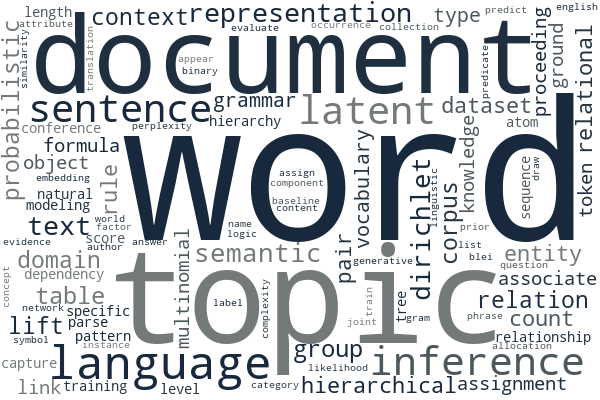
\includegraphics[width=\linewidth]{01.Chapters/05.Results/pres_00}
		\caption{Present topic number 0.}
	\end{subfigure}%
	\hfill
	\begin{subfigure}{0.49\textwidth}
		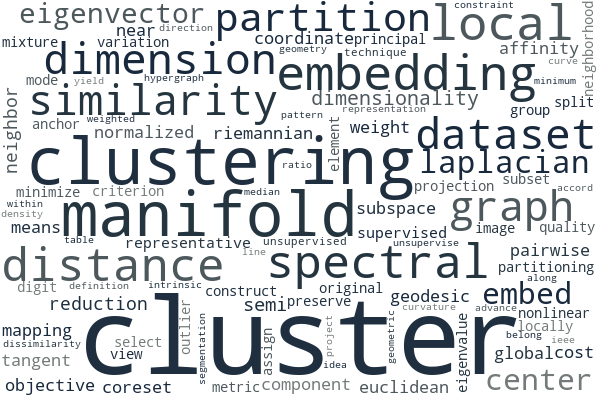
\includegraphics[width=\linewidth]{01.Chapters/05.Results/pres_13}
		\caption{Present topic number 13.}
	\end{subfigure}%
	\vfill
	\begin{subfigure}{0.49\textwidth}
		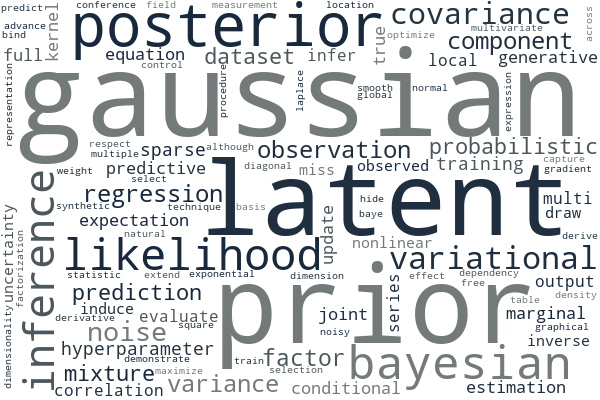
\includegraphics[width=\linewidth]{01.Chapters/05.Results/pres_16}
		\caption{Present topic number 16.}
	\end{subfigure}%
	\hfill
	\begin{subfigure}{0.49\textwidth}
		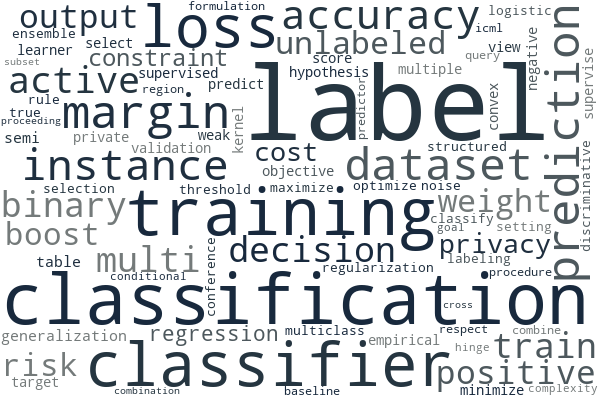
\includegraphics[width=\linewidth]{01.Chapters/05.Results/pres_24}
		\caption{Present topic number 24.}
	\end{subfigure}%
	\caption{\textit{Present} topics wordclouds.}
	\label{fig:pres-wordcloud}
\end{figure}

Figures \ref{fig:pres-topic-dist} and \ref{fig:pres-topic-per-doc} have the same idea as the Figures \ref{fig:past-topic-dist} and \ref{fig:past-topic-per-doc}. The \ref{fig:pres-topic-dist} shows that the topics are well distributed over the documents, the topic present in more documents is about $35\%$ of them. Figure \ref{fig:pres-topic-per-doc} shows the distribution of \textit{present} topics over the docuements, similarly to the \textit{past} distribution, the documents have mostly about 3 and 4 topics and none of then have more than 10 topics.

\begin{figure}[h!]
	\begin{subfigure}{0.49\textwidth}
		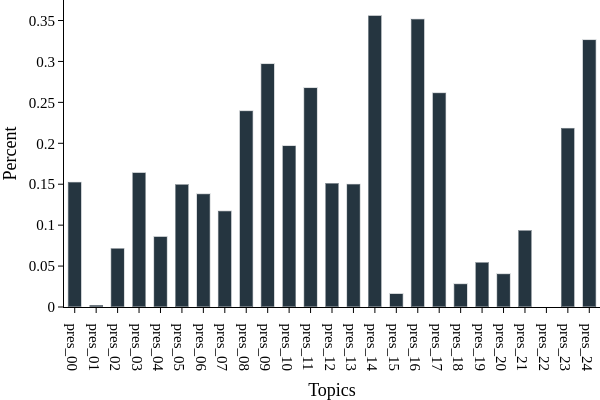
\includegraphics[width=\linewidth]{01.Chapters/05.Results/pres-percentage-bar}
		\caption{Percentage of documents with topics.}
		\label{fig:pres-percentage-bar}
	\end{subfigure}%
	\hfill
	\begin{subfigure}{0.49\textwidth}
		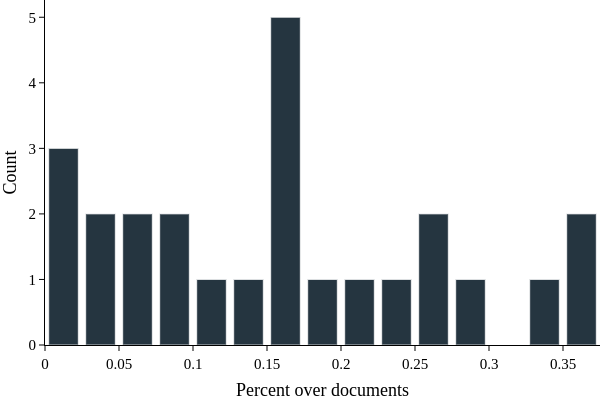
\includegraphics[width=\linewidth]{01.Chapters/05.Results/pres-percentage-hist}
		\caption{Histogram for the topic percentages.}
		\label{fig:pres-percentage-hist}
	\end{subfigure}%
	\caption{Distribution of topics over the documents.}
	\label{fig:pres-topic-dist}
\end{figure}

\begin{figure}[h!]
	\centering
	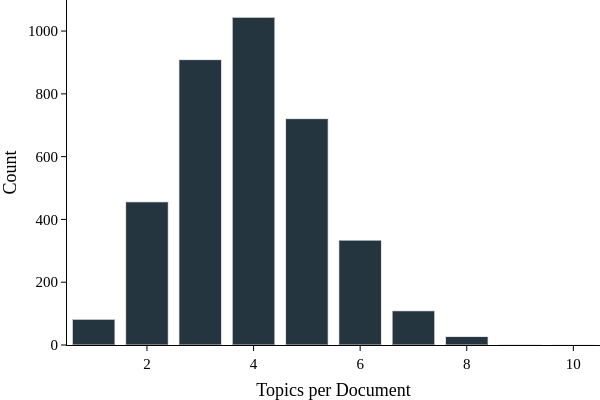
\includegraphics[width=0.6\linewidth]{01.Chapters/05.Results/pres-topic-per-doc}
	\caption{Histogram for the number of topics per document.}
	\label{fig:pres-topic-per-doc}
\end{figure}

\subsection{Past-Present Combination}

With the \textit{past} and \textit{present} topics defined, the similarity metrics described in section \ref{sec:material-combination} were applied to obtain the topic correspondence. For $\text{Sim}_{1}$, we use the top 50 words, i.e., $N=50$. As $\text{Sim}_{1}$ and $\text{Sim}_{2}$ are negatively correlated, to aggregate then, we divide $\text{Sim}_{1}$ for $\text{Sim}_{2}$ to capture the best from both metrics. Table \ref{tab:correspondence-score} illustrates the main correspondences between \textit{past} and \textit{present} topics.

\begin{table}[h!]
	\centering
	\caption{Main association for \textit{past} and \textit{present} topics.}
	\label{tab:correspondence-score}
	\begin{tabular}{cc|ccc}
		\toprule
		\textbf{Past} & \textbf{Present} & \textbf{$\text{Sim}_{1}$} & \textbf{$\text{Sim}_{2}$} & \textbf{$\text{Sim}_{1} / \text{Sim}_{2}$} \\ \midrule
		 11  &  06  & 58\% & 0.026 & 1119.71 \\
		 10  &  05  & 56\% & 0.031 & 911.39  \\
		 14  &  16  & 44\% & 0.040 & 555.48  \\
		 20  &  09  & 38\% & 0.036 & 528.22  \\
		 18  &  11  & 40\% & 0.043 & 467.59  \\
		 07  &  12  & 34\% & 0.038 & 445.64  \\
		 04  &  02  & 54\% & 0.061 & 440.94  \\
		 00  &  08  & 46\% & 0.055 & 417.94  \\
		 05  &  03  & 32\% & 0.047 & 341.65  \\
		 22  &  07  & 36\% & 0.057 & 313.72  \\ \bottomrule
	\end{tabular}
\end{table}

By aggregating the two metrics, we are choosing topics whose common word distribution is similar while giving priority to topics with the most similar top words. For example, take the combinations 18-11 and 07-12, the second one is the closest in terms of word distribution, but the first has the top 50 more similar making this combination stronger. Table \ref{tab:correspondence-words} shows the intersection for those top 10 topic combinations.

\begin{table}[h!]
	\centering
	\caption{Words intersection for the main combinations.}
	\label{tab:correspondence-words}
	\begin{tabular}{cc|lllll}
		\toprule
		\textbf{Present} & \textbf{Past} & \multicolumn{5}{c}{\textbf{Words}} \\ \midrule
		11 & 06 & neuron   & spike      & cell        & response   & stimulus      \\
		10 & 05 & policy   & action     & control     & reward     & reinforcement \\
		14 & 16 & gaussian & mixture    & likelihood  & prior      & bayesian      \\
		20 & 09 & gradient & constraint & convergence & update     & cost          \\
		18 & 11 & bound    & theorem    & loss        & bind       & proof         \\
		07 & 12 & subject  & stimulus   & human       & response   & trial         \\
		04 & 02 & signal   & filter     & noise       & frequency  & channel       \\
		00 & 08 & object   & image      & recognition & pixel      & shape         \\
		05 & 03 & markov   & inference  & sequence    & likelihood & bayesian      \\
		22 & 07 & unit     & training   & layer       & train      & hide          \\ \bottomrule
	\end{tabular}
\end{table}

Through the intersections we see that the topics of the \textit{past} continued in the \textit{present}. For example, the combination 10-05 talks about reinforcement learning, and 22-07 is about deep learning. From that, we evaluate how the models of the \textit{past} behave with the \textit{present}.

\section{Document Classification}

This section will cover the results behind the classification model. First, the training process and model selection with the \textit{Past} set, then, the evaluation of those models at \textit{Present} according to the combination of topics.

\subsection{Model Selection}

%With the documents labeled, we now have our \textit{Labeled Past} dataset. From that, we can train a binary classification model for each topic. For the classification was performed cross-validation with 10 folds for each combination of vectorization + model, the raw results for those models are in Appendix \ref{apdx:classification}.

We now have the \textit{Labeled Past} dataset. From that, we can train a classification model for each topic. For this was performed cross-validation with 10 folds for each combination of vectorization + model, the raw results for those models are in Appendix \ref{apdx:classification}.

%To evaluate which model is the best, we will compare the average of the model scores for all topics. Table \ref{tab:classification-report} shows the comparison between the precision, recall and f1 score for the models. As marked in the table, the best model is the XXXX with XXXX.

To evaluate which model is the best, we will compare the average of the model scores for all topics. Table \ref{tab:classification-report} shows the comparison between the precision, recall, and f1 for the models.
As marked in the table, the best model is the TF-IDF with SVM.

\begin{table}[h!]
	\centering
	\caption{Classification models comparison.}
	\label{tab:classification-report}
	\begin{tabular}{c|ccc}
		\toprule
		\multirow{2}{*}{\textbf{Type}} & \multicolumn{3}{c}{\textbf{Statistics}} \\\cmidrule{2-4}
		 & \textbf{Precision} & \textbf{Recall} & \textbf{F1 Score} \\ \midrule
		\multicolumn{1}{l|}{BOW + Naive Bayes}     & 0.656 & 0.781 & 0.695 \\
		\multicolumn{1}{l|}{TF-IDF + Naive Bayes}  & 0.719 & 0.483 & 0.553 \\
		\multicolumn{1}{l|}{BOW + SVM}             & 0.863 & 0.539 & 0.648 \\
		\multicolumn{1}{l|}{\textbf{TF-IDF + SVM}} & \textbf{0.906} & \textbf{0.683} & \textbf{0.769} \\
%		\multicolumn{1}{l|}{GloVe + SVM}        & - & - & - \\
		\bottomrule
	\end{tabular}
\end{table}

Following these results, we identified that we have a bias for higher precision than recall. These results show us the models tend not to predict more positive classes than the existent ones, on the other hand, the smaller recall indicates the models are mispredicting the documents that really belongs to that class. Tables \ref{tab:nb-bow} to \ref{tab:svm-tfidf}, from Appendix \ref{apdx:classification}, also show the more imbalanced the class, the predictions tend to be less accurate.


\subsection{Evaluating Present Predictions}

With the built classifiers from the \textit{Labeled Past} set, we apply it in the \textit{present} set and compare the output with its labels. Using just the top-10 combinations in Table \ref{tab:correspondence-score} we have obtained the average results for this predictions shown in Table \ref{tab:avg-combination-score} below.

\begin{table}[h!]
	\centering
	\caption{Metrics for the top-10 topic combinations.}
	\label{tab:avg-combination-score}
	\begin{tabular}{cc|ccc}
		\toprule
		\textbf{Past} & \textbf{Present} & \textbf{Precision} & \textbf{Recall} & \textbf{F1 Score} \\ \midrule
		11 & 06 & 0.976 & 0.563 & 0.714 \\
		10 & 05 & 0.936 & 0.709 & 0.807 \\
		14 & 16 & 0.640 & 0.697 & 0.667 \\
		20 & 09 & 0.699 & 0.547 & 0.614 \\
		18 & 11 & 0.552 & 0.795 & 0.651 \\
		07 & 12 & 0.790 & 0.249 & 0.379 \\
		04 & 02 & 0.454 & 0.355 & 0.398 \\
		00 & 08 & 0.967 & 0.368 & 0.533 \\
		05 & 03 & 0.324 & 0.820 & 0.464 \\
		22 & 07 & 0.680 & 0.550 & 0.608 \\
		\bottomrule
	\end{tabular}
\end{table}

In addition to this comparison, we want to evaluate the behavior of the models over the years. For this, we will evaluate the f1 score for each year isolated. In Figure \ref{fig:f1-combination} is presented the charts for them over the years, Figure \ref{fig:top1-5} shows the first to fifth, and Figure \ref{fig:top6-10} shows the remaining combinations.

\begin{figure}[h!]
	\begin{subfigure}{0.49\textwidth}
		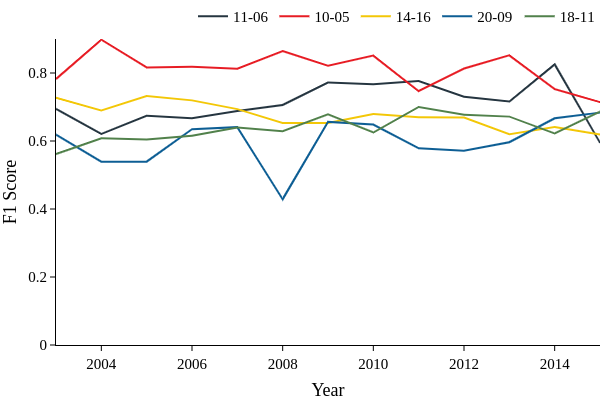
\includegraphics[width=\linewidth]{01.Chapters/05.Results/f1-combination-1-5}
		\caption{Combinations 1 to 5.}
		\label{fig:top1-5}
	\end{subfigure}%
	\hfill
	\begin{subfigure}{0.49\textwidth}
		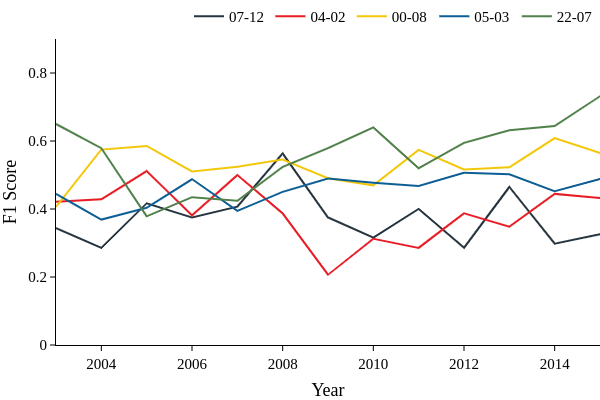
\includegraphics[width=\linewidth]{01.Chapters/05.Results/f1-combination-6-10}
		\caption{Combinations 6 to 10.}
		\label{fig:top6-10}
	\end{subfigure}%
	\caption{F1 Score for the main combinations.}
	\label{fig:f1-combination}
\end{figure}


% Comentar resultados das tabelas e dos gráficos
From Table \ref{tab:avg-combination-score}, we see a high negative correlation between the position of combinations and their f1 scores, $-0.775$ for the record. This result said to us that is a decreasing relationship between the predictions of these combinations. Figure \ref{fig:combination-corr} shows a scatter plot for this relationship with an ordinary least squares (OLS) trend line.

\begin{figure}[h!]
	\centering
	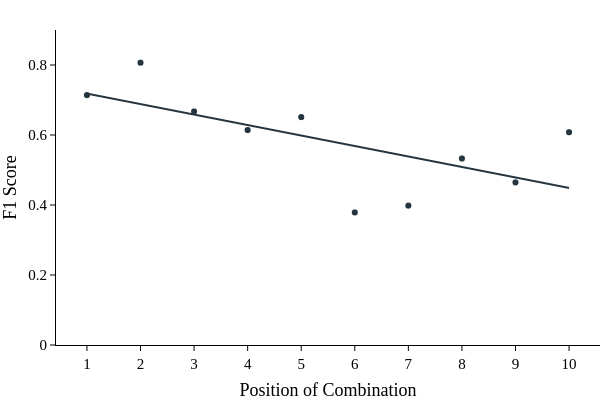
\includegraphics[width=0.6\linewidth]{01.Chapters/05.Results/combination-corr}
	\caption{F1 Score correlation with the combination position.}
	\label{fig:combination-corr}
\end{figure}

This decreasing trend reflects directly in score curves in Figure \ref{fig:f1-combination}. Despite slight fluctuations, the decreasing trend in combinations scores could indicate that even in the best combinations the predictions are not so accurate. The terms evolution over the years to develop the topics maybe have changed and the models can not learn these new terms.

Let us observe a little deeper at the relationship between the score and the time evolution. In Figure \ref{fig:isolated-topics} we have a scatter plot with the local regression trendline of LOWESS type for the two best combinations. Notice that despite a small increase, there is a natural tendency of constancy followed by a decrease in the models' efficiency over the years. Again, this inclination suggests that the rising of new terms for new techniques affects the classification.

\begin{figure}[h!]
	\begin{subfigure}{0.5\textwidth}
	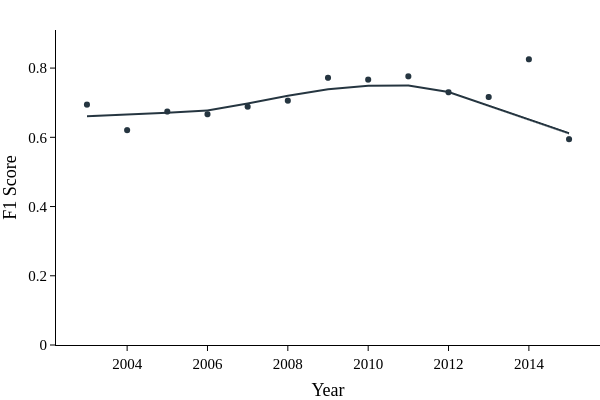
\includegraphics[width=\linewidth]{01.Chapters/05.Results/lowess-1}
		\caption{Topics combination \textit{Past 11} - \textit{Present 06}.}
	\end{subfigure}%
	\hfill
	\begin{subfigure}{0.5\textwidth}
		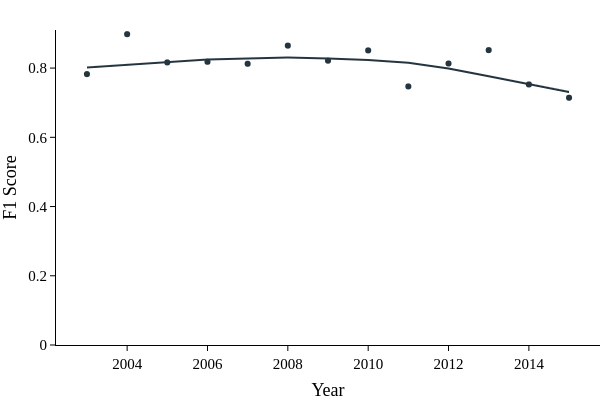
\includegraphics[width=\linewidth]{01.Chapters/05.Results/lowess-2}
		\caption{Topics combination \textit{Past 10} - \textit{Present 05}.}
	\end{subfigure}%
	\caption{F1 Score for the main combinations.}
	\label{fig:isolated-topics}
\end{figure}

\newpage
Realize that combinations under the top 5 may have some growth trend. However, in general, these combinations already have low efficiency in relation to the best ones, decreasing the result's reliability.


